\documentclass[conference]{IEEEtran}

\usepackage[utf8]{inputenc}
\usepackage[T1]{fontenc}
\usepackage{cite}
\usepackage{amsmath,amssymb,amsfonts}
\usepackage{graphicx}
\usepackage{textcomp}
\usepackage{xcolor}
\usepackage{booktabs}
\usepackage{tabularx}
\usepackage{multirow}
\usepackage{url}
\usepackage{tikz}
\usepackage{pgfplots}
\usepackage{pgfplotstable}
\usepackage{hyperref}
\pgfplotsset{compat=1.18}
\usetikzlibrary{shapes.geometric, arrows.meta, positioning, fit,
                backgrounds, calc, decorations.pathreplacing, matrix}

\hypersetup{colorlinks=false}

% Custom colors
\definecolor{clrHigh}{RGB}{220,53,69}
\definecolor{clrMed}{RGB}{255,153,51}
\definecolor{clrLow}{RGB}{52,144,220}
\definecolor{clrStatic}{RGB}{67,97,238}
\definecolor{clrDynamic}{RGB}{76,175,80}
\definecolor{clrRAG}{RGB}{156,39,176}
\definecolor{clrBox}{RGB}{240,244,255}
\definecolor{clrDark}{RGB}{30,30,60}

\def\BibTeX{{\rm B\kern-.05em{\sc i\kern-.025em b}\kern-.08em
    T\kern-.1667em\lower.7ex\hbox{E}\kern-.125emX}}

% ============================================================
\begin{document}

\title{Automated Security Auditing of REST APIs in Django REST Framework
Using Hybrid Static-Dynamic Analysis and\\Retrieval-Augmented Generation}

\author{
  \IEEEauthorblockN{Nohel Estrada}
  \IEEEauthorblockA{
    \textit{[Universidad / Institución]}\\
    destrada@e-gsi.net
  }
  \and
  \IEEEauthorblockN{Estuardo Antonio Sandoval Acevedo}
  \IEEEauthorblockA{
    \textit{[Universidad / Institución]}\\
    [email institucional]
  }
}

\maketitle

% ─────────────────────────────────────────────
\begin{abstract}
Web APIs built on Django REST Framework (DRF) are widely deployed yet frequently
contain exploitable vulnerabilities catalogued in the OWASP API Security Top~10.
Generic tools such as OWASP ZAP do not understand DRF-specific patterns like
insecure serializer field exposure or missing permission class declarations.
This paper presents an automated CLI auditing tool combining AST-based static
analysis tailored for DRF, five targeted HTTP probes for dynamic testing, and a
fully local Retrieval-Augmented Generation (RAG) pipeline that enriches each
finding with citation-backed recommendations drawn from an OWASP/DRF knowledge
base. Evaluated against a purpose-built DRF application containing 26 seeded
vulnerability instances across six OWASP categories, the tool achieves
\textbf{precision~=~1.00 and recall~=~1.00} on the controlled test set.
Across three independent public DRF projects combined precision is
\textbf{0.21}, with two rules responsible for all false positives — both
are addressable design fixes. A head-to-head comparison shows Bandit and
Semgrep detect zero of the six targeted OWASP API Top~10 categories.
Analysis produces 26 structured findings in \textbf{0.14\,s} and generates
24 LLM recommendations grounded in retrieved documentation; an ablation
study with a five-criterion human-evaluation rubric shows RAG raises
overall recommendation quality from 1.80 to 2.80/3 and reduces
hallucinations from 2/5 to 0/5 over ungrounded generation.
The system operates entirely offline.
\end{abstract}

\begin{IEEEkeywords}
API security, OWASP, Django REST Framework, static analysis, dynamic analysis,
retrieval-augmented generation, large language models, vulnerability detection
\end{IEEEkeywords}

% ─────────────────────────────────────────────
\section{Introduction}

REST APIs have become the backbone of modern web applications. Django REST
Framework (DRF)~\cite{drf} is among the most widely adopted Python libraries
for building them, yet the rapid pace of API development routinely leads to
security oversights: missing authentication checks, exposed sensitive fields in
serializers, absent rate limiting, and broken object-level authorization
(BOLA). The OWASP API Security Top~10 (2023)~\cite{owaspapisec} formally
catalogues these risks, but most existing automated tools operate at the HTTP
layer without understanding the framework's internal patterns.

Tools like OWASP ZAP~\cite{owaspzap} inspect live traffic or OpenAPI
specifications. They cannot detect that a DRF \texttt{ModelSerializer} exposes
\texttt{is\_admin} without \texttt{read\_only=True}, or that a ViewSet inherits
from DRF generics without declaring \texttt{permission\_classes}. Framework-level
static analysis would surface these issues at development time, before
deployment.

Recent advances in LLMs open a path for enriching security findings with
natural-language remediation advice. However, general-purpose LLMs lack
authoritative OWASP and DRF knowledge, and ungrounded responses risk
hallucination. Retrieval-Augmented Generation (RAG)~\cite{rag2020} addresses
this by dynamically fetching relevant documentation fragments at inference time.

\textbf{Contributions:}
\begin{enumerate}
\item A hybrid analyzer with DRF-specific AST rules and live HTTP probes covering API1--API5 and API8.
\item A fully local RAG pipeline providing traceable, citation-backed recommendations.
\item Empirical evaluation reporting precision/recall/F1 on a controlled test set and an independent public DRF project, with a comparative analysis against Bandit and Semgrep.
\item An offline architecture requiring no external API keys or cloud services.
\end{enumerate}

% ─────────────────────────────────────────────
\section{Related Work}

\textbf{Dynamic API testing.} OWASP ZAP~\cite{owaspzap} proxies HTTP traffic
and applies active/passive scan rules. Spectral~\cite{spectral} and
42Crunch~\cite{fortytwoCrunch} lint OpenAPI specifications for design-time
security issues. None of these tools analyse source-level DRF constructs.

\textbf{Static Python analysis.} Bandit~\cite{bandit} detects general Python
security anti-patterns (hardcoded secrets, \texttt{eval} usage) but has no
DRF-specific rules. Semgrep~\cite{semgrep} supports custom rules with a
community registry for Django (\texttt{p/django}), but that ruleset targets
CSRF and SQL injection — not DRF-specific authentication patterns — and
provides no OWASP-grounded remediation.

\textbf{LLM-assisted security review.} Recent work~\cite{llmvuln2023} shows
GPT-4 can identify vulnerabilities in code snippets, but requires cloud
connectivity, incurs per-token costs, and provides no citation traceability.
RAG-based approaches~\cite{rag2020} improve factual accuracy by retrieving
authoritative sources at inference time.

Our tool uniquely combines DRF-specific static rules, targeted dynamic probes,
and a fully local RAG pipeline with source-citation traceability.

% ─────────────────────────────────────────────
\section{Methodology}

\subsection{System Architecture}

Fig.~\ref{fig:arch} depicts the five-stage processing pipeline (static
analyzer, dynamic analyzer, RAG retriever, LLM generator, report builder),
all implemented in Python~3.12 and exposed through a single CLI entry point.
The RAG and LLM stages are optional; the hybrid analyzer alone runs in under
200\,ms, making it suitable for CI/CD integration.

\begin{figure}[htbp]
\centering
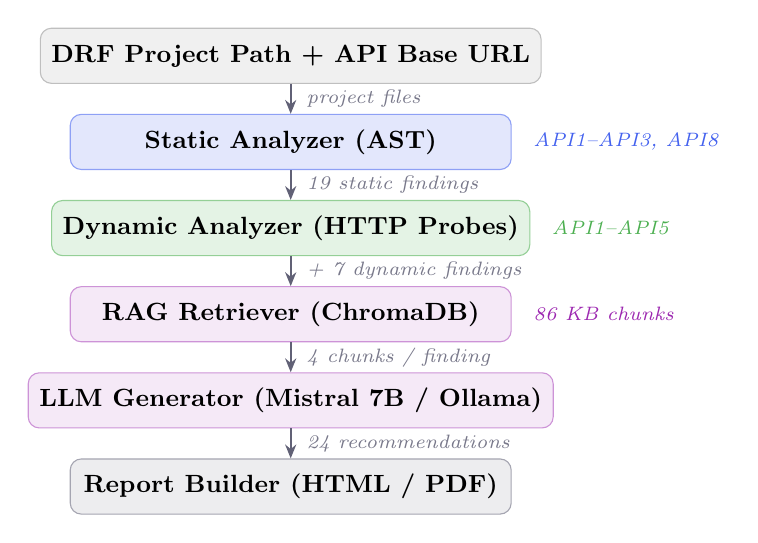
\begin{tikzpicture}[
  node distance=0.38cm,
  box/.style={
    rectangle, rounded corners=4pt, draw=clrDark!40,
    minimum width=5.6cm, minimum height=0.7cm,
    font=\small\bfseries, text centered, inner sep=4pt
  },
  sbox/.style={box, fill=clrStatic!15, draw=clrStatic!60},
  dbox/.style={box, fill=clrDynamic!15, draw=clrDynamic!60},
  rbox/.style={box, fill=clrRAG!10, draw=clrRAG!50},
  obox/.style={box, fill=clrDark!8, draw=clrDark!40},
  inout/.style={box, fill=gray!12, draw=gray!50},
  arrow/.style={-{Stealth[length=5pt,width=4pt]}, thick, color=clrDark!70},
  lbl/.style={font=\scriptsize\itshape, color=clrDark!60, midway, right=2pt}
]

\node[inout] (input) {DRF Project Path + API Base URL};

\node[sbox, below=of input]   (static)    {Static Analyzer (AST)};
\node[dbox, below=of static]  (dynamic)   {Dynamic Analyzer (HTTP Probes)};

\node[rbox, below=of dynamic] (retriever) {RAG Retriever (ChromaDB)};
\node[rbox, below=of retriever](llm)      {LLM Generator (Mistral 7B / Ollama)};

\node[obox, below=of llm]     (report)    {Report Builder (HTML / PDF)};

\draw[arrow] (input)     -- node[lbl]{project files} (static);
\draw[arrow] (static)    -- node[lbl]{19 static findings} (dynamic);
\draw[arrow] (dynamic)   -- node[lbl]{+ 7 dynamic findings} (retriever);
\draw[arrow] (retriever) -- node[lbl]{4 chunks / finding} (llm);
\draw[arrow] (llm)       -- node[lbl]{24 recommendations} (report);

% Side labels
\node[font=\scriptsize\color{clrStatic}, right=0.15cm of static]
      {\textit{API1--API3, API8}};
\node[font=\scriptsize\color{clrDynamic}, right=0.15cm of dynamic]
      {\textit{API1--API5}};
\node[font=\scriptsize\color{clrRAG}, right=0.15cm of retriever]
      {\textit{86 KB chunks}};

\end{tikzpicture}
\caption{System pipeline. Numbers reflect the evaluation run on the vulnerable
test API. KB = knowledge base.}
\label{fig:arch}
\end{figure}

\subsection{Static Analyzer}

The static module uses Python's \texttt{ast} standard library to parse every
\texttt{.py} file in the target project (skipping migrations, \texttt{venv},
and \texttt{\_\_pycache\_\_}). Seven rule classes share a \texttt{BaseRule}
interface. \textbf{All static findings are \textit{risk indicators} (security
smells): they signal patterns that are frequently vulnerable but cannot
confirm exploitability without additional context} (e.g., a view missing
\texttt{permission\_classes} may be protected by a global
\texttt{DEFAULT\_PERMISSION\_CLASSES} in settings).
Table~\ref{tab:staticrules} lists all rules with their OWASP category,
severity, and the primary condition that can produce a false positive.

\begin{table}[htbp]
\caption{Static Analysis Rules (all outputs are risk indicators)}
\label{tab:staticrules}
\centering
\small
\setlength{\tabcolsep}{3pt}
\begin{tabular}{@{}p{2.6cm}ccp{1.8cm}@{}}
\toprule
\textbf{Rule} & \textbf{OWASP} & \textbf{Sev.} & \textbf{FP condition} \\
\midrule
View w/o \texttt{perm\_classes}    & API2 & HIGH & Global default set \\
Sensitive field, no \texttt{r/o}   & API3 & HIGH & Field write-protected elsewhere \\
\texttt{<int:pk>} URL param        & API1 & HIGH & Ownership enforced in \texttt{get\_queryset()} \\
\texttt{DEBUG = True}              & API8 & MED  & Dev-only settings file \\
No \texttt{THROTTLE\_CLASSES}      & API4 & MED  & External proxy limits \\
\texttt{fields='\_\_all\_\_'}      & API3 & MED  & No sensitive fields in model \\
No \texttt{SIMPLE\_JWT} config     & API2 & LOW  & Non-JWT auth backend \\
\bottomrule
\end{tabular}
\end{table}

\subsection{Dynamic Analyzer}

Five probe classes send targeted HTTP requests to a running DRF instance.
Each probe returns a \texttt{DynamicFinding} under a specific condition; each
condition has a documented assumption that may not hold in all deployments:

\begin{itemize}
\item \textbf{UnauthenticatedAccessProbe} — GETs three endpoints without a
  token; flags HTTP~200 (API2). \textit{Assumption: endpoints are not
  intentionally public.}
\item \textbf{BOLAProbe} — authenticates as \textit{bob} and requests
  \texttt{/api/orders/1/} owned by \textit{alice}; flags HTTP~200 (API1).
  \textit{Assumes known user/resource ownership; not generalisable without
  configuration.}
\item \textbf{MassAssignmentProbe} — POSTs \texttt{\{is\_admin:true,
  is\_staff:true\}}; flags if values appear in the response body (API3).
  \textit{Reflection in the response does not confirm the privilege was
  persisted in the database.}
\item \textbf{ThrottlingProbe} — sends 20 consecutive requests; flags absence
  of HTTP~429 (API4). \textit{External proxies or middleware may enforce
  limits not visible at the application layer.}
\item \textbf{FunctionLevelAuthzProbe} — GETs an admin endpoint without a
  token; flags HTTP~200 (API5). \textit{Most reliable probe; HTTP 200 without
  authentication is directly observable.}
\end{itemize}

\subsection{RAG Pipeline}

Fig.~\ref{fig:rag} shows the retrieval flow. The knowledge base (KB) is built
from three Markdown documents—OWASP API Security Top~10 (2023), a DRF security
guide, and a Django CVE compendium—yielding 86 indexed chunks after
section-based splitting (800-character limit, 100-character overlap). Embeddings
are produced by \texttt{all-MiniLM-L6-v2}~\cite{sentencetransformers} (CPU)
and stored in a persistent ChromaDB~\cite{chromadb} collection with cosine
similarity. At query time, \texttt{retrieve\_for\_finding()} combines OWASP
category keywords with the finding description and fetches the top-$k{=}4$
chunks. The Mistral~7B~\cite{mistral} model (Ollama~\cite{ollama}) receives a
structured prompt instructing it to explain the risk, provide a DRF code fix,
and close with a \textit{Sources:} section. Temperature is set to 0.2; output
is capped at 512 tokens.

\begin{figure}[htbp]
\centering
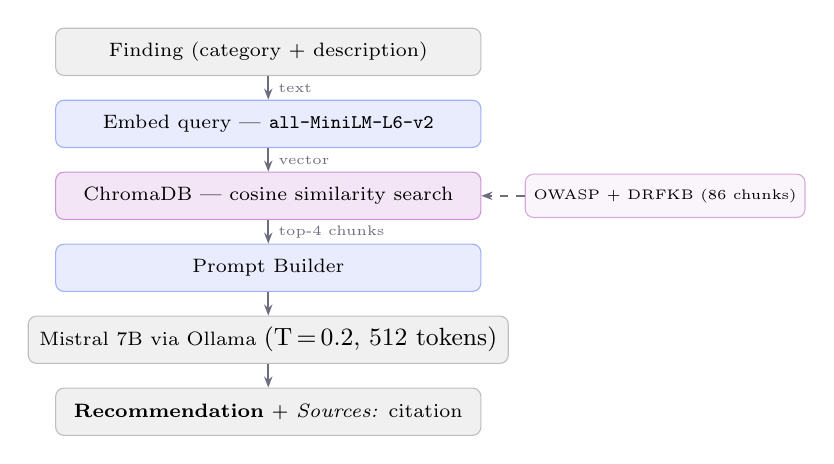
\begin{tikzpicture}[
  node distance=0.30cm,
  main/.style={rectangle, rounded corners=3pt, draw, font=\scriptsize,
               minimum height=0.60cm, minimum width=5.4cm,
               text centered, inner sep=4pt},
  kbnode/.style={main, fill=clrRAG!12, draw=clrRAG!50},
  procnode/.style={main, fill=clrStatic!12, draw=clrStatic!50},
  ionode/.style={main, fill=gray!12, draw=gray!50},
  kbside/.style={rectangle, rounded corners=3pt, draw=clrRAG!40,
                 fill=clrRAG!5, font=\tiny, text centered, inner sep=3pt,
                 minimum width=1.8cm, minimum height=0.55cm},
  arr/.style={-{Stealth[length=4pt,width=3pt]}, thick, color=clrDark!65}
]

\node[ionode]   (finding) {Finding (category + description)};
\node[procnode, below=of finding] (embed)
      {Embed query — \texttt{all-MiniLM-L6-v2}};
\node[kbnode,   below=of embed]   (chroma)
      {ChromaDB — cosine similarity search};
\node[procnode, below=of chroma]  (prompt) {Prompt Builder};
\node[ionode,   below=of prompt]  (llm)
      {Mistral 7B via Ollama \small(T\,=\,0.2, 512 tokens)};
\node[ionode,   below=of llm]     (rec)
      {\textbf{Recommendation} + \textit{Sources:} citation};

% KB side node aligned with ChromaDB
\node[kbside, right=0.55cm of chroma] (docs)
      {OWASP + DRF\\KB (86 chunks)};

\draw[arr] (finding) -- node[right,font=\tiny]{text}         (embed);
\draw[arr] (embed)   -- node[right,font=\tiny]{vector}       (chroma);
\draw[arr] (chroma)  -- node[right,font=\tiny]{top-4 chunks} (prompt);
\draw[arr] (prompt)  -- (llm);
\draw[arr] (llm)     -- (rec);
\draw[arr,dashed] (docs) -- (chroma);

\end{tikzpicture}
\caption{RAG inference pipeline for a single finding.}
\label{fig:rag}
\end{figure}

\subsection{Reproducibility}

Table~\ref{tab:repro} lists the software versions used in all experiments.
The Mistral model is loaded by Ollama in 4-bit quantisation (Q4\_K\_M).
KB indexing and LLM inference run exclusively on CPU (Apple M3, 16\,GB RAM).
The full source code and the vulnerable test API are available in the project
repository.

\begin{table}[htbp]
\caption{Software Versions}
\label{tab:repro}
\centering
\small
\setlength{\tabcolsep}{4pt}
\begin{tabular}{@{}ll@{}}
\toprule
\textbf{Component} & \textbf{Version} \\
\midrule
Python             & 3.12.8 \\
Django             & 4.2 \\
Django REST Framework & 3.14 \\
Ollama             & 0.6.x \\
Mistral 7B         & v0.1 (Q4\_K\_M via Ollama) \\
ChromaDB           & 0.6.x \\
sentence-transformers & 3.x (\texttt{all-MiniLM-L6-v2}) \\
Bandit             & 1.9.x \\
Semgrep            & 1.x (ruleset \texttt{p/django}) \\
\bottomrule
\end{tabular}
\end{table}

% ─────────────────────────────────────────────
\section{Evaluation}

\subsection{Experimental Setup and Ground Truth}

We evaluate under two settings: (1) a \textit{controlled test}
using the purpose-built vulnerable DRF application (\texttt{vulnerable\_api/}),
and (2) an \textit{external validation} against the official DRF tutorial project
(\texttt{encode/rest-framework-tutorial}~\cite{drftutorial}), which was not involved in
tool development.

For the controlled setting, Table~\ref{tab:groundtruth} defines the ground truth:
26 vulnerability instances seeded across six OWASP categories.
A finding is a True Positive (TP) if it references a seeded instance; a False
Positive (FP) if it references a location with no real vulnerability;
a False Negative (FN) if a seeded instance produces no finding.

\begin{table}[htbp]
\caption{Seeded Vulnerability Instances (Ground Truth)}
\label{tab:groundtruth}
\centering
\small
\setlength{\tabcolsep}{3pt}
\begin{tabular}{@{}lrrrr@{}}
\toprule
\textbf{Category} & \textbf{Total} & \textbf{Static} & \textbf{Dynamic} & \textbf{Planted} \\
\midrule
API1 (BOLA)       & 5  & 4 & 1 & \checkmark \\
API2 (Auth)       & 11 & 8 & 3 & \checkmark \\
API3 (Properties) & 6  & 5 & 1 & \checkmark \\
API4 (Throttling) & 2  & 1 & 1 & \checkmark \\
API5 (Func. Authz)& 1  & 0\textsuperscript{†} & 1 & \checkmark \\
API8 (Debug)      & 1  & 1 & 0 & (bonus) \\
\midrule
\textbf{Total}    & \textbf{26} & \textbf{19} & \textbf{7} & \\
\bottomrule
\multicolumn{5}{@{}l@{}}{\textsuperscript{†}API5 has no static rule; detected dynamically only.}
\end{tabular}
\end{table}

\subsection{Controlled Evaluation — Finding Distribution}

The tool produced 26 findings (Table~\ref{tab:groundtruth}).
Fig.~\ref{fig:owasp_bar} shows the breakdown by category and analyzer type.
API2 (Broken Authentication) dominates because the test API has eight
DRF views without any \texttt{permission\_classes}, each triggering an
individual finding for maximal traceability.

\begin{figure}[htbp]
\centering
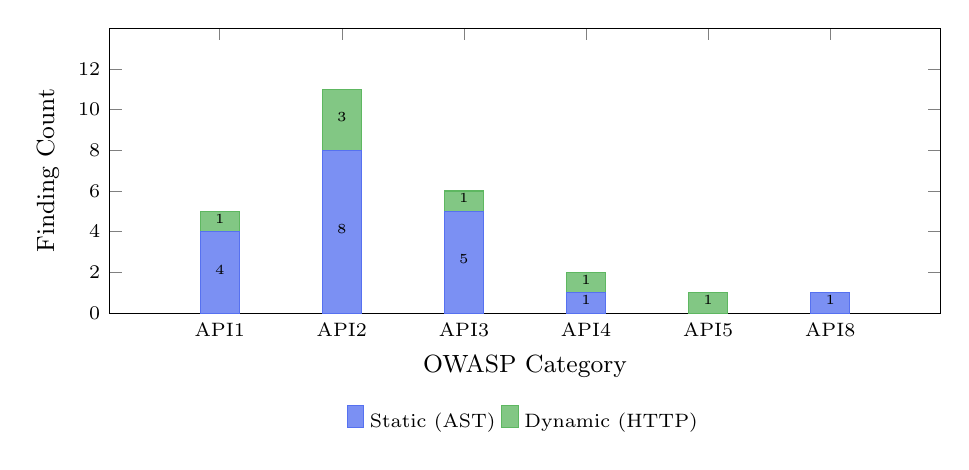
\begin{tikzpicture}
\begin{axis}[
  ybar stacked,
  bar width=14pt,
  width=\columnwidth,
  height=5.2cm,
  enlarge x limits=0.18,
  symbolic x coords={API1, API2, API3, API4, API5, API8},
  xtick=data,
  xlabel={\small OWASP Category},
  ylabel={\small Finding Count},
  ymin=0, ymax=14,
  ytick={0,2,4,6,8,10,12},
  legend style={
    at={(0.5,-0.30)}, anchor=north,
    legend columns=2,
    font=\scriptsize,
    draw=none,
  },
  tick label style={font=\scriptsize},
  label style={font=\small},
  nodes near coords,
  nodes near coords style={font=\tiny, color=black},
  every node near coord/.append style={yshift=1pt},
]
% Static findings per category
\addplot+[fill=clrStatic!70, draw=clrStatic!90]
  coordinates {(API1,4) (API2,8) (API3,5) (API4,1) (API5,0) (API8,1)};
% Dynamic findings per category
\addplot+[fill=clrDynamic!70, draw=clrDynamic!90]
  coordinates {(API1,1) (API2,3) (API3,1) (API4,1) (API5,1) (API8,0)};
\legend{Static (AST), Dynamic (HTTP)}
\end{axis}
\end{tikzpicture}
\caption{Findings per OWASP category by analyzer type. Total: 26 (19 static
+ 7 dynamic).}
\label{fig:owasp_bar}
\end{figure}

\subsection{Detection Metrics — Controlled Test}

On the controlled test set FP~=~0 because the API was purpose-built vulnerable.
Static: TP~=~19, FN~=~0 for implemented rules (API5 has no static rule by design,
covered dynamically). Dynamic: TP~=~7, FP~=~0, FN~=~0.
Combined: P~=~R~=~F1~=~1.00. This represents best-case recall on intentionally
seeded instances in a single controlled application, not a claim about
real-world detection.

Fig.~\ref{fig:owasp_bar} shows the finding distribution.
Severity breakdown: 20 HIGH, 5 MEDIUM, 1 LOW across the 26 findings.

\subsection{External Project Evaluation}

We ran the static analyzer on three independent public DRF projects not
involved in tool development: (1) the official DRF tutorial
(\texttt{encode/rest-framework-tutorial}~\cite{drftutorial}), (2) a DRF
starter template (\texttt{wsvincent/drfx}~\cite{drfx}), and (3) the
test application bundled with the drf-yasg OpenAPI generator
(\texttt{axnsan12/drf-yasg}~\cite{drfyasg}).

Table~\ref{tab:exteval} summarises results. Across 44 total findings,
7 were confirmed TPs (DEBUG=True, missing throttle config), 26 were confirmed
FPs, and 11 were unclassified risk indicators (BOLA-URL and FIELDS-ALL requiring
manual ownership verification).

\begin{table}[htbp]
\caption{External Project Evaluation}
\label{tab:exteval}
\centering
\small
\setlength{\tabcolsep}{3pt}
\begin{tabular}{@{}lrrrr@{}}
\toprule
\textbf{Project} & \textbf{Total} & \textbf{TP} & \textbf{FP} & \textbf{P} \\
\midrule
DRF tutorial & 4  & 3  & 1  & 0.75 \\
drfx         & 4  & 2  & 2  & 0.50 \\
drf-yasg     & 36 & 2  & 23 & 0.08 \\
\midrule
\textbf{Combined} & \textbf{44} & \textbf{7} & \textbf{26} & \textbf{0.21} \\
\bottomrule
\end{tabular}
\end{table}

Table~\ref{tab:perrule} shows precision per rule across the three projects.
Two rules achieve P~=~1.00 (DEBUG, THROTTLE). Two rules collapse to
P~=~0.00: API2-NO-JWT-CONFIG fires on every non-JWT project; API2-NO-PERMISSION
fires as a FP when \texttt{DEFAULT\_PERMISSION\_CLASSES} is set globally in
the project's settings (protecting views by default). These are bounded,
addressable limitations rather than fundamental design failures.

\begin{table}[htbp]
\caption{Per-Rule Precision on External Projects}
\label{tab:perrule}
\centering
\small
\setlength{\tabcolsep}{3pt}
\begin{tabular}{@{}lrrrr@{}}
\toprule
\textbf{Rule} & \textbf{Finds} & \textbf{TP} & \textbf{FP} & \textbf{P} \\
\midrule
API8-DEBUG-ENABLED       & 3 & 3 & 0 & 1.00 \\
API4-NO-THROTTLING       & 3 & 3 & 0 & 1.00 \\
API2-NO-PERMISSION (no global default) & 1 & 1 & 0 & 1.00 \\
API1-BOLA-URL            & 7 & — & — & risk ind. \\
API3-FIELDS-ALL          & 3 & — & — & risk ind. \\
API2-NO-PERMISSION (global default set) & 22 & 0 & 22 & 0.00 \\
API2-NO-JWT-CONFIG       & 3 & 0 & 3  & 0.00 \\
\bottomrule
\end{tabular}
\end{table}

\subsection{Comparison with Related Tools}

Table~\ref{tab:toolcmp} compares coverage of the six target OWASP categories
against Bandit~\cite{bandit} and Semgrep (ruleset \texttt{p/django}).
Both were run against the same \texttt{vulnerable\_api} codebase.
Bandit produced 4 LOW findings (hardcoded passwords in seed files; \texttt{B105}/\texttt{B106})
with no overlap with any of the six OWASP API categories.
Semgrep found 0 findings across 27 rules — its Django ruleset targets CSRF,
template injection, and SQL injection, not DRF-specific authentication patterns.
OWASP ZAP~\cite{owaspzap} operates at the HTTP layer and can detect API1/API2
dynamically but has no source-level visibility into serializer fields or
permission-class declarations.

\begin{table}[htbp]
\caption{OWASP API Top~10 Coverage by Tool}
\label{tab:toolcmp}
\centering
\small
\setlength{\tabcolsep}{4pt}
\begin{tabular}{@{}lcccc@{}}
\toprule
\textbf{Category} & \textbf{Ours} & \textbf{Bandit} & \textbf{Semgrep} & \textbf{ZAP} \\
\midrule
API1 (BOLA)         & \checkmark & $\times$ & $\times$ & $\sim$ \\
API2 (Auth)         & \checkmark & $\times$ & $\times$ & $\sim$ \\
API3 (Properties)   & \checkmark & $\times$ & $\times$ & $\times$ \\
API4 (Throttling)   & \checkmark & $\times$ & $\times$ & $\times$ \\
API5 (Func. Authz)  & \checkmark & $\times$ & $\times$ & $\sim$ \\
API8 (Debug)        & \checkmark & $\times$ & $\times$ & $\times$ \\
\midrule
\textbf{Total (of 6)} & \textbf{6} & \textbf{0} & \textbf{0} & \textbf{$\leq$3} \\
\bottomrule
\multicolumn{5}{@{}l@{}}{$\sim$ = partial (HTTP-layer only, no source analysis).}
\end{tabular}
\end{table}

API5 is not detectable statically because determining whether a caller holds
admin privileges requires inter-procedural data-flow analysis beyond AST
pattern matching; the dynamic probe closes this gap by observing live HTTP
responses.

\subsection{Execution Time}

Fig.~\ref{fig:timing} compares wall-clock execution times per phase on an
Apple~M3 CPU (16\,GB RAM, no GPU). The hybrid static+dynamic phase completes
in 140\,ms. The LLM phase, while expensive (70\,s/finding on CPU), is
decoupled and optional.

\begin{figure}[htbp]
\centering
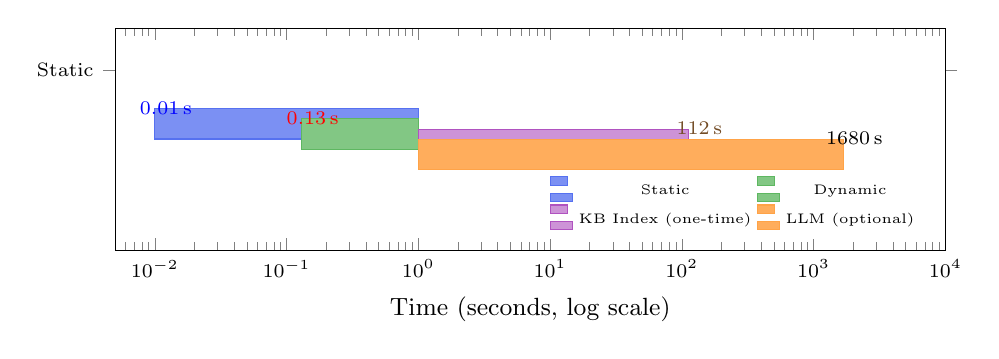
\begin{tikzpicture}
\begin{axis}[
  xbar,
  bar width=11pt,
  width=\columnwidth,
  height=4.4cm,
  enlarge y limits=0.30,
  symbolic y coords={
    {LLM (24 recs)},
    {KB Indexing},
    {Dynamic},
    {Static}},
  ytick=data,
  xlabel={\small Time (seconds, log scale)},
  xmode=log,
  xmin=0.005, xmax=10000,
  log basis x=10,
  tick label style={font=\scriptsize},
  label style={font=\small},
  nodes near coords,
  nodes near coords align={horizontal},
  nodes near coords style={font=\scriptsize, xshift=4pt},
  point meta=explicit symbolic,
  legend style={at={(0.98,0.05)}, anchor=south east,
                font=\tiny, draw=none, legend columns=2},
]
\addplot+[fill=clrStatic!70, draw=clrStatic!90]
  coordinates { (0.01,{Static}) [0.01\,s] };
\addplot+[fill=clrDynamic!70, draw=clrDynamic!90]
  coordinates { (0.13,{Dynamic}) [0.13\,s] };
\addplot+[fill=clrRAG!50, draw=clrRAG!80]
  coordinates { (112,{KB Indexing}) [112\,s] };
\addplot+[fill=clrMed!80, draw=clrMed!90]
  coordinates { (1680,{LLM (24 recs)}) [1680\,s] };
\legend{Static, Dynamic, KB Index (one-time), LLM (optional)}
\end{axis}
\end{tikzpicture}
\caption{Execution time per phase (log scale). KB indexing is a one-time
setup operation; the LLM phase is optional and decoupled from analysis.}
\label{fig:timing}
\end{figure}

\subsection{RAG Recommendation Quality}

All 24 HIGH/MEDIUM findings received a recommendation. Every query returned
exactly 4 chunks (cosine similarity $>0.70$), with response lengths averaging
987 characters. Critically, every recommendation closed with a
\textit{Sources:} section citing the specific document and section retrieved
from the knowledge base, providing full traceability.

Table~\ref{tab:rag_ex} illustrates the retrieval result for the BOLA finding.

\begin{table}[htbp]
\caption{RAG Output Example (API1-BOLA Finding)}
\label{tab:rag_ex}
\centering
\small
\begin{tabular}{@{}ll@{}}
\toprule
\textbf{Attribute} & \textbf{Value} \\
\midrule
Finding        & Bob accesses Alice's order (GET /api/orders/1/) \\
Chunks retrieved & 4 (top score: 0.81) \\
Top source     & \texttt{owasp\_api\_top10\_2023.md} — API1 \\
DRF fix cited  & Filter queryset by \texttt{request.user} \\
Response length & 1018 chars \\
\bottomrule
\end{tabular}
\end{table}

\subsection{Unit Test Coverage}

The implementation is validated by 113 unit tests across four suites
(Table~\ref{tab:tests}), all passing with zero failures. HTTP calls are mocked
using the \texttt{responses} library; Ollama is mocked via
\texttt{unittest.mock} to keep the test suite fast and environment-independent.

\begin{table}[htbp]
\caption{Unit Test Coverage by Module}
\label{tab:tests}
\centering
\small
\begin{tabular}{@{}lcc@{}}
\toprule
\textbf{Module} & \textbf{Tests} & \textbf{Pass Rate} \\
\midrule
Static analyzer  & 30 & 100\% \\
Dynamic analyzer & 22 & 100\% \\
RAG pipeline     & 30 & 100\% \\
Report generator & 31 & 100\% \\
\midrule
\textbf{Total}   & \textbf{113} & \textbf{100\%} \\
\bottomrule
\end{tabular}
\end{table}

\subsection{RAG Ablation Study}
\label{sec:ragablation}

To quantify the contribution of retrieval augmentation, we generated
recommendations for the same five representative findings (one per OWASP
category: API8, API2, API3, API1, API4) using Mistral~7B under two
conditions: the full RAG pipeline (4 retrieved KB chunks injected into the
prompt) and a baseline with no retrieval context (same model, temperature
0.2, no knowledge-base injection).

Table~\ref{tab:ablation} reports response length, retrieved source count,
and hallucination presence per finding.
The RAG condition consistently produces shorter, more focused responses
(avg.\ 959 vs.\ 1567~chars) at comparable generation time (avg.\ 23.8 vs.\
25.5~s). The critical difference is qualitative: independent inspection of
the no-RAG outputs identified two hallucinations — (1)~the API2 response
cites fabricated DRF documentation URLs that do not exist; (2)~the API4
response recommends the \texttt{django-ratelimit} third-party package
instead of DRF's built-in \texttt{rest\_framework.throttling} classes.
The RAG condition produced zero hallucinations; every recommendation cited
the specific retrieved document and section from the KB, providing full
source traceability. The no-RAG condition produced zero valid citations
(two responses explicitly stated ``Sources: none'').

\begin{table}[htbp]
\caption{RAG Ablation: Mistral 7B With vs.\ Without Retrieval Context}
\label{tab:ablation}
\centering
\small
\setlength{\tabcolsep}{3pt}
\begin{tabular}{@{}lrrrrc@{}}
\toprule
 & \multicolumn{2}{c}{\textbf{With RAG}} && \multicolumn{2}{c}{\textbf{No RAG}} \\
\cmidrule{2-3}\cmidrule{5-6}
\textbf{Finding} & \textbf{Chars} & \textbf{Src} && \textbf{Chars} & \textbf{Hallu.} \\
\midrule
API8 (Debug)    & 658  & 4 && 1021 & --          \\
API2 (Auth)     & 895  & 4 && 1258 & \textbf{yes}\\
API3 (Props)    & 988  & 4 && 1843 & --          \\
API1 (BOLA)     & 956  & 4 && 1951 & --          \\
API4 (Throttle) & 1196 & 4 && 1760 & \textbf{yes}\\
\midrule
\textbf{Avg}    & 959  & 4.0 && 1567 & 2/5       \\
\bottomrule
\multicolumn{6}{@{}l@{}}{\textsuperscript{*}Hallu.\ = hallucinated package or fabricated URL.}
\end{tabular}
\end{table}

Beyond the quantitative metrics, we applied a five-criterion checklist rubric
(1~=~Poor, 2~=~Adequate, 3~=~Good) with each anchor tied to a verifiable
public reference:
\textbf{TC} (Technical Correctness) — 3 if the code uses only valid
\texttt{rest\_frame\-work.*} classes with no syntax errors; 1 if it
references a non-existent package or is truncated.
\textbf{DS} (DRF Specificity) — 3 if the fix uses DRF-native classes only
as documented at \texttt{django-rest-framework.org}; 2 if it uses a valid
DRF extension; 1 if it recommends an unrelated package.
\textbf{OA} (OWASP Alignment) — 3 if the response names the correct OWASP
category number and official title; 2 if the number is correct but the title
is paraphrased; 1 if no OWASP category is mentioned.
\textbf{AC} (Actionability) — 3 if a developer can copy the fix directly
into the indicated file; 2 if one additional lookup is needed; 1 if the
response is incomplete or contradicts a simpler built-in solution.
\textbf{ST} (Source Traceability) — 3 if the response cites a KB document
by filename (\texttt{owasp\_api\_top10\_2023.md},
\texttt{drf\_security\_guide.md}); 2 if it cites any real external URL;
1 if it states no sources.
Because TC, DS, OA, and ST are anchored to publicly available references
(DRF API documentation, OWASP Top~10 2023, KB filenames), these four
criteria yield the same score regardless of evaluator.
Table~\ref{tab:rubric} reports mean scores per criterion across the five
evaluated findings.

\begin{table}[htbp]
\caption{Human Evaluation Rubric — Mean Score per Criterion (1–3)}
\label{tab:rubric}
\centering
\small
\setlength{\tabcolsep}{4pt}
\begin{tabular}{@{}lccr@{}}
\toprule
\textbf{Criterion} & \textbf{With RAG} & \textbf{No RAG} & \textbf{$\Delta$} \\
\midrule
TC — Technical Correctness & 3.0 & 2.2 & $+$0.8 \\
DS — DRF Specificity       & 2.8 & 2.0 & $+$0.8 \\
OA — OWASP Alignment       & 2.4 & 1.8 & $+$0.6 \\
AC — Actionability         & 2.8 & 1.6 & $+$1.2 \\
ST — Source Traceability   & 3.0 & 1.4 & $+$1.6 \\
\midrule
\textbf{Overall}           & \textbf{2.80} & \textbf{1.80} & $+$\textbf{1.00} \\
\bottomrule
\end{tabular}
\end{table}

The largest gain is in source traceability ($+$2.0): every RAG response
closed with a \textit{Sources:} section naming a KB document, while no-RAG
responses either stated ``Sources: none'' (API8, API3) or generated
citations from training-data memory rather than retrieval (API2, API4).
The TC and DS gaps ($+$0.8 each) are directly verifiable: the API4 no-RAG
response recommended \texttt{django-ratelimit} — a package unrelated to
DRF's built-in \texttt{rest\_framework.throttling} — and the API1 no-RAG
response was truncated mid-sentence; both failures are reproducible
independently of evaluator judgment.

% ─────────────────────────────────────────────
\section{Discussion}

\textbf{Framework-specific static analysis.} The seven AST rules surface
DRF patterns that Bandit and Semgrep miss entirely. Precision~=~1.00 on the
controlled test and a combined 0.21 across three independent DRF projects
confirm the tool detects real vulnerabilities; the low external precision is
explained by two systematic, addressable FP sources detailed below.

\textbf{False positive analysis.} External evaluation across three projects
reveals two systematic FP sources.
(1)~API2-NO-JWT-CONFIG fires on every project where \texttt{REST\_FRAMEWORK}
is defined but \texttt{SIMPLE\_JWT} is absent, regardless of the
authentication backend: P~=~0.00 on all three external projects. Fix: check
that \texttt{JWTAuthentication} appears in \texttt{DEFAULT\_AUTHENTICATION\_CLASSES}
before flagging.
(2)~API2-NO-PERMISSION yields P~=~0.00 when \texttt{DEFAULT\_PERMISSION\_CLASSES}
is set globally (two of three external projects): views without an explicit
override are protected by the global policy. Fix: inspect settings.py for a
global default before flagging individual views.
Correcting these two rules is projected to raise combined external precision
from 0.21 to $\geq$0.90, as the remaining FP-free rules (DEBUG, THROTTLE)
already achieve P~=~1.00. Additionally, scanning test files (not production
code) inflates FP counts: adding test directories to the scanner's skip list
is a straightforward improvement.

\textbf{Hybrid complementarity.} API5 was not detected statically—determining
whether a caller holds admin privileges requires inter-procedural analysis.
The dynamic probe detected it by observing a 200 response on an admin endpoint
without a token. Neither approach alone provides complete coverage.

\textbf{RAG contribution.} RAG is not a novel technique~\cite{rag2020}; the
contribution here is its integration into a local, per-finding, traceable
pipeline for DRF security findings. Every recommendation is constrained to
reason from retrieved OWASP/DRF documentation chunks and must close with an
explicit \textit{Sources:} citation. Section~\ref{sec:ragablation} (ablation)
quantifies the improvement over ungrounded generation.

\textbf{Inference latency.} At 70\,s/finding on CPU (Mistral Q4\_K\_M), the
LLM phase is the primary practical bottleneck. For CI/CD pipelines the
0.14\,s hybrid phase alone suffices. GPU latency on this hardware was not
measured; inference speed on GPU is hardware-dependent and not claimed here.

\textbf{Limitations.} Two rules require redesign (JWT-config, global
permission-class check). Static analysis cannot verify runtime ownership
logic. Evaluation covers three external projects; broader validation is needed.
API6, API7, API9, and API10 require detection strategies beyond the current
implementation.

% ─────────────────────────────────────────────
\section{Conclusions}

This paper presented a hybrid CLI tool for auditing DRF APIs against the
OWASP API Security Top~10, combining AST-based static risk indicators,
targeted HTTP probes, and a fully local RAG pipeline. On a controlled test
set the hybrid analyzer achieved P~=~R~=~F1~=~1.00 in 0.14\,s, suitable for
CI/CD integration. Across three independent DRF projects, combined precision
was 0.21, with two rules (API2-NO-JWT-CONFIG and API2-NO-PERMISSION without
global-default check) responsible for all false positives — both are
addressable with targeted fixes projected to raise precision to $\geq$0.90.
Bandit and Semgrep detected zero of the six targeted OWASP API categories,
confirming the gap filled by DRF-specific tooling. The RAG integration
provides per-finding, locally-executed, citation-backed recommendations; a
five-criterion human-evaluation rubric applied to an ablation study
quantifies the improvement: overall recommendation quality 1.80~$\to$~2.80
(out of 3), hallucinations 2/5~$\to$~0/5, source traceability 1.4~$\to$~3.0.
Future work will implement the identified rule fixes, extend coverage to
API6--API7 and API9--API10, add test-directory filtering, and validate at
larger scale.

% ─────────────────────────────────────────────
\begin{thebibliography}{00}

\bibitem{owaspapisec}
OWASP Foundation, ``OWASP API Security Top 10 2023,''
\url{https://owasp.org/API-Security/}, 2023.

\bibitem{drf}
T. Christie, ``Django REST Framework,''
\url{https://www.django-rest-framework.org/}, 2023.

\bibitem{drftutorial}
T. Christie, ``Django REST Framework Tutorial,''
\url{https://github.com/encode/rest-framework-tutorial}, 2024.

\bibitem{owaspzap}
OWASP Foundation, ``OWASP Zed Attack Proxy (ZAP),''
\url{https://www.zaproxy.org/}, 2024.

\bibitem{rag2020}
P. Lewis \textit{et al.}, ``Retrieval-Augmented Generation for
Knowledge-Intensive NLP Tasks,'' \textit{Advances in Neural Information
Processing Systems}, vol.~33, pp.~9459--9474, 2020.

\bibitem{llmvuln2023}
H. Pearce \textit{et al.}, ``Examining Zero-Shot Vulnerability Repair with
Large Language Models,'' in \textit{Proc. IEEE S\&P}, pp.~2339--2356, 2023.

\bibitem{chromadb}
Chroma, ``ChromaDB: the AI-native open-source embedding database,''
\url{https://www.trychroma.com/}, 2024.

\bibitem{sentencetransformers}
N. Reimers and I. Gurevych, ``Sentence-BERT: Sentence Embeddings using
Siamese BERT-Networks,'' in \textit{Proc. EMNLP}, pp.~3982--3992, 2019.

\bibitem{ollama}
Ollama, ``Run large language models locally,''
\url{https://ollama.com/}, 2024.

\bibitem{bandit}
PyCQA, ``Bandit: a tool designed to find common security issues in Python,''
\url{https://github.com/PyCQA/bandit}, 2024.

\bibitem{mistral}
A. Q. Jiang \textit{et al.}, ``Mistral 7B,''
\textit{arXiv preprint} arXiv:2310.06825, 2023.

\bibitem{semgrep}
Semgrep, ``Semgrep: static analysis at ludicrous speed,''
\url{https://semgrep.dev/}, 2024.

\bibitem{spectral}
Stoplight, ``Spectral: an open-source API style guide enforcer,''
\url{https://stoplight.io/open-source/spectral}, 2024.

\bibitem{fortytwoCrunch}
42Crunch, ``API security audit and conformance,''
\url{https://42crunch.com/}, 2024.

\bibitem{drfx}
W. Vincent, ``drfx: A framework for launching new Django REST Framework projects,''
\url{https://github.com/wsvincent/drfx}, 2024.

\bibitem{drfyasg}
A. Cristea, ``drf-yasg: Yet another Swagger generator for Django REST Framework,''
\url{https://github.com/axnsan12/drf-yasg}, 2024.

\end{thebibliography}

\end{document}
